\subsection{PolyPassHash Extensions}
\label{sec-extensions}

There are three major limitations of PolyPassHash as described in the previous
section.   
First, for some systems like Facebook or gmail, an attacker may control a
huge number of accounts.  In practice there are really two 
types of accounts: those that should count toward the threshold (likely 
administrators or power users) and those that should not.   This section
describes an extension to support ``thresholdless'' accounts that do not 
count toward the threshold.
Second, there is not a way to handle non-password authentication schemes
like biometrics, private key authentication, etc.   This section 
discusses how to integrate into existing mechanisms.   
Third, the system
must have a threshold of correct passwords before any can be authenticated.
This may cause logins to be delayed for an unacceptable time after a restart.
This section discusses an extension that leaks partial information about salted 
password hashes, but allows immediate authentication upon restart.   As a 
result, PolyPassHash still provides an exponential security increase, but 
no longer must wait for account logins upon restart.




\subsubsection{Thresholdless Accounts}
\label{sec-thresholdless}

A desirable property is the ability to handle user accounts that should
not count toward the threshold.  For example, gmail and Facebook have 
a huge number of users that are untrusted and can create their accounts 
automatically.   None of these user accounts, no matter how many, should be
allowed to count toward the threshold for verifying other accounts.   

We will support accounts that should not count toward the threshold by
computing their salted hash and then encrypting this data with
a symmetric cryptographic cipher (AES).   If the server knows the AES key, 
it can clearly authenticate thresholdless users.
However, if the AES key is stored on
disk, an attacker that compromises the password file could compromise the
AES key too.   

To protect the AES key while stored on disk we will use a slightly modified
version of the PolyHashing store algorithm.   This store is identical to 
the main algorithm except
that the lowest order term (the constant term) of the polynomial represents 
a portion of the encryption key, as is shown in the bottom half of 
Figure~\ref{fig-polypasshashoverview}.   (The key is stored in the same manner
as traditional Shamir Secret Sharing
where the constant term of the Polynomial encodes the secret.)
A party that knows the threshold of administrator passwords can XOR those
values to recover sufficient shares to reconstruct the polynomial (and thus
the key).  
By the properties of Shamir Secret Sharing, the key has information-theoretic 
privacy from an attacker unless they possess a threshold of account passwords.



Creation of a thresholdless account involves a similar series of steps to
other PolyPassHash passwords.   As before the system obtains the 
salted hash for the password.   However, the salted cryptographic hash of 
the password is encrypted with AES instead of XORing it with a share.
To indicate this is a thresholdless account, the share field can 
be set to 0 to indicate that this is not a normal PolyPassHash 
store.   (Note that the share 0 will not be used normally in Shamir secret
sharing.)   When the user attempts to login, if a large enough 
threshold of passwords has been entered, the AES key is available to decrypt 
the hash, allowing the user to  be authenticated.   However,
if the stored threshold data is disclosed, it is not useful to an attacker
unless they can recover the AES key by knowing a threshold of
administrator passwords.


If desired by an administrator, accounts can be switched between thresholdless
and threshold without user intervention.
In both the case of threshold and thresholdless accounts, a server with
a threshold of shares knows the information necessary to recover the salted 
secure hash.   This salted secure hash can then be re-encoded in the 
alternative manner and the new entry can be stored.

\subsubsection{Handling Alternative Authentication Mechanisms}

Passwords are not the only mechanism for logging into modern systems.   For
example, it is common for users to use a private key to login over {\tt
ssh}, biometric-based authentication holds substantial promise, 
smart cards are often used to hide user credentials, and single
sign-in systems like OAuth and OpenID are commonplace and provided by 
many major websites.   Any practical protection mechanism needs to operate
in conjunction with such techniques.

Handling non-password login for \emph{thresholdless} user accounts is trivial 
because
it requires no changes to the system.   Non-password login can be handled 
using the existing login mechanisms without any modification.
This is especially important for techniques like OAuth and OpenID which 
are almost certainly not going to be used to protect administrator accounts
(which count toward the threshold), but will be desirable to average users.

For administrator accounts or other accounts which are expected to contribute
to the threshold, one must devise other techniques.   Fortunately there is
a significant amount of prior work on secure remote authentication and
techniques for using this to hide 
secrets~\cite{deo1998authentication, yang1999password}.   This can be used to 
protect the Shamir Secret Share(s) for the account.
It is possible to view the authentication as decrypting information using a 
secret stored by a remote party (as in fact many such systems are implemented).
We can encrypt the Shamir Secret Share for the user with their key and then
check that the resulting $x$ and $f(x)$ are correct for the user.   

For example, suppose that an administrator has a private key that they use
to login (as is common with SSH private key authentication or smart card
based authentication).   Instead of
XORing the Shamir share with the salted hash of the password, it can
be encrypted with the user's public key.   When the administrator presents
their key to login, this key is used to decrypt the original share.   This
process can be repeated multiple times if the user has multiple shares.
 The share can then be used the same as any other share to 
unlock a PolyPassHash data store.


For authentication of threshold account using other techniques such as 
biometrics, there has been prior work on deriving a private key from this 
(noisy) data~\cite{juels2006fuzzy}.   Once a key is derived from the biometric 
data, the scheme will function identically to the private key authentication 
scheme discussed above.




\subsubsection{Partial Verification}
\label{sec-partial}

When a PolyHashing store restarts, no values may be authenticated until a
threshold are provided.   If the time delay is not important and the rate
at which values are provided is rapid, this may not pose a problem.   However,
in many scenarios, this delay may prove burdensome.

This issue can be addressed with a technique called \emph{partial 
verification}.   Partial verification has the password database
leak partial information about the hash to allow verification before a threshold
is reached.   The core idea is similar for threshold accounts and 
thresholdless accounts, but for simplicity will be explained with threshold
accounts first.   If the Shamir Secret Share is chosen so that it is shorter
than the hash value, this will leak some bytes of the salted hash.
The `partial' hash that is leaked can be used for verification purposes.


\begin{figure}[t]
\center
% We need pdflatex with png images. Plain latex would fail here.
% So, we conditionally include this so we can still build with latex,
% just without this image.
%\begin{minipage}[b]{\linewidth}
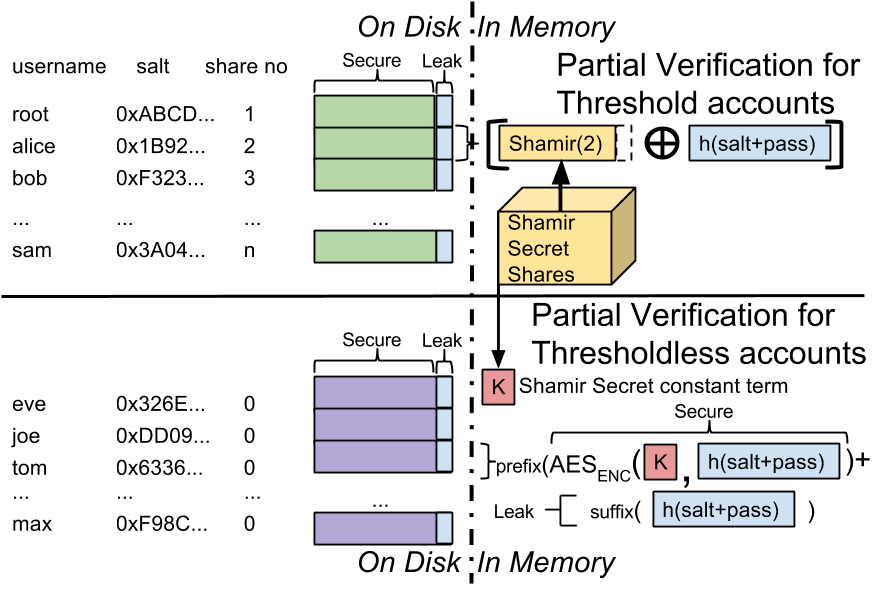
\includegraphics[width=1.05\columnwidth]{figures/partialverification.png}
%\end{minipage}
\caption{This figure shows validation using partial verification.
A portion of suffix of the salted hash is stored on disk.  This
allows verification of accounts before a threshold of correct passwords is
provided.
}
\label{fig-partialverification}
\end{figure}

For example, suppose there is a 32 byte salted hash and a 30 byte 
secret (Figure~\ref{fig-partialverification}).   The secret will XOR with
the first 30 bytes, effectively obscuring them.   However, the remaining
2 bytes will consist of the suffix of the salted hash.   When the
system restarts, accounts can be validated using the last 2 bytes of the
hash.   Once sufficient accounts have logged in, the full
hash can be recovered and account authorizations can be 
performed using the full hash as was described in the 
previous section.

Thresholdless accounts can also be validated before a threshold is reached
if partial validation is used.   The technique is similar to threshold 
accounts, where a portion of the suffix of the hash replaces
some of the encrypted hash on disk.   Validation can be 
performed with the suffix until a threshold of correct passwords are provided
and the Shamir Secret Store (and thus the AES key) are recovered.

Increasing the length of the hash which is leaked has a negative 
effect on the resulting data store security.
First of all, suppose that $l$ bits are leaked with via the hash.
This allows an attacker that compromises the password hash database to 
discard $2^l$ possibilities from the password search space.   Thus
if there is a threshold of $k$ and each password has $n$ bits of entropy, 
the attacker can make $k$ passes of cost $2^n$ to remove all but $2^{n-l}$
passwords.   Following this, the attacker will then need to simultaneously
guess from the remaining passwords which will cost an additional $2^{k*(n-l)}$
to crack the store.   (Section~\ref{sec-feasibility} discusses the practical
impact this has on password security.)

However, a small hash also has a negative ramification that
incorrect passwords could log in before a threshold is reached.   In fact,
the probability of a random password working is $\frac{1}{2}^l$.   Rate
limiting the rate of password attempts can mitigate the risk from an attacker
that does not know the salt.   However, if an attacker has stolen the password 
database, they can quickly compute a value that will be correctly verified 
upon restart.  However, once a threshold of passwords is provided,
PolyPassHash knows the full hash and can detect any such
malicious logins.   Much like other decoy schemes~\cite{juels2013honeywords,
Kontaxis_CCS_2013}, partial verification allow incorrect logins but
later detects this occurrence and provides strong evidence that the password
database was leaked.

\eat{
The length of the leaked information need not be the same for every 
account.   There is no reason why the threshold and thresholdless accounts
need to have the same length of leaked information.   In fact, every 
thresholdless account could have a unique quantity of leaked information,
perhaps to take into account entropy in the password.   For threshold
accounts, a variable amount of leaked information could be appended to each
share.   Since the shares hide the secret, leaking hash
information effectively leaks some parts of the shares to the attacker.
We will study the security implications of leaking variable portions of 
threshold accounts in future work.

}





